\documentclass[a4paper,11pt]{article}
\usepackage{amsmath,amsthm,amsfonts,amssymb,amscd,amstext,vmargin,graphics,graphicx,tabularx,multicol} 
\usepackage[francais]{babel}
\usepackage[utf8]{inputenc}  
\usepackage[T1]{fontenc} 
\usepackage{pstricks-add,tikz,tkz-tab,variations}
\usepackage[autolanguage,np]{numprint} 

\setmarginsrb{1.5cm}{0.5cm}{1cm}{0.5cm}{0cm}{0cm}{0cm}{0cm} %Gauche, haut, droite, haut
\newcounter{numexo}
\newcommand{\exo}[1]{\stepcounter{numexo}\noindent{\bf Exercice~\thenumexo} : \marginpar{\hfill /#1}}
\reversemarginpar


\newcounter{enumtabi}
\newcounter{enumtaba}
\newcommand{\q}{\stepcounter{enumtabi} \theenumtabi.  }
\newcommand{\qa}{\stepcounter{enumtaba} (\alph{enumtaba}) }
\newcommand{\initq}{\setcounter{enumtabi}{0}}
\newcommand{\initqa}{\setcounter{enumtaba}{0}}

\newcommand{\be}{\begin{enumerate}}
\newcommand{\ee}{\end{enumerate}}
\newcommand{\bi}{\begin{itemize}}
\newcommand{\ei}{\end{itemize}}
\newcommand{\bp}{\begin{pspicture*}}
\newcommand{\ep}{\end{pspicture*}}
\newcommand{\bt}{\begin{tabular}}
\newcommand{\et}{\end{tabular}}
\renewcommand{\tabularxcolumn}[1]{>{\centering}m{#1}} %(colonne m{} centrée, au lieu de p par défault) 
\newcommand{\tnl}{\tabularnewline}

\newcommand{\bmul}[1]{\begin{multicols}{#1}}
\newcommand{\emul}{\end{multicols}}

\newcommand{\trait}{\noindent \rule{\linewidth}{0.2mm}}
\newcommand{\hs}[1]{\hspace{#1}}
\newcommand{\vs}[1]{\vspace{#1}}

\newcommand{\N}{\mathbb{N}}
\newcommand{\Z}{\mathbb{Z}}
\newcommand{\R}{\mathbb{R}}
\newcommand{\C}{\mathbb{C}}
\newcommand{\Dcal}{\mathcal{D}}
\newcommand{\Ccal}{\mathcal{C}}
\newcommand{\mc}{\mathcal}

\newcommand{\vect}[1]{\overrightarrow{#1}}
\newcommand{\ds}{\displaystyle}
\newcommand{\eq}{\quad \Leftrightarrow \quad}
\newcommand{\vecti}{\vec{\imath}}
\newcommand{\vectj}{\vec{\jmath}}
\newcommand{\Oij}{(O;\vec{\imath}, \vec{\jmath})}
\newcommand{\OIJ}{(O;I,J)}


\newcommand{\reponse}[1][1]{%
\multido{}{#1}{\makebox[\linewidth]{\rule[0pt]{0pt}{20pt}\dotfill}
}}

\newcommand{\titre}[5] 
% #1: titre #2: haut gauche #3: bas gauche #4: haut droite #5: bas droite
{
\noindent #2 \hfill #4 \\
#3 \hfill #5

\vspace{-1.6cm}

\begin{center}\rule{6cm}{0.5mm}\end{center}
\vspace{0.2cm}
\begin{center}{\large{\textbf{#1}}}\end{center}
\begin{center}\rule{6cm}{0.5mm}\end{center}
}



\begin{document}
\pagestyle{empty}
\titre{Contrôle 1}{Nom :}{Prénom :}{Classe}{Date}

\begin{flushleft}
\begin{tabular}{|m{9.5cm}|m{1.25cm}|m{1.25cm}|m{1.25cm}|m{1.25cm}|m{1.25cm}|}
\hline 
\textbf{Compétences} & \begin{center}
\textbf{N.E.}
\end{center} & \begin{center}
\textbf{M.I.}
\end{center} & \begin{center}
\textbf{M.F.}
\end{center}  & \begin{center}
\textbf{M.S.}
\end{center} & \begin{center}
\textbf{T.B.M.}
\end{center} \\ 
\hline 
Je dois savoir traduire en langage mathématique une situation réelle &  &  & & &\\
\hline 
Je dois savoir démontrer : utiliser un raisonnement logique et des règles établies (propriétés, théorèmes, formules) pour parvenir à une conclusion&  &  & & &\\
\hline
Je dois respecter les priorités de calculs  &  &  & & &\\ 
\hline


\end{tabular} 
\end{flushleft}

\textit{N.E = Non évalué ; M.I. = Maîtrise insuffisante ; M.F. = Maîtrise fragile ; M.S. = Maîtrise satisfaisante ; T.B.M. = Très bonne maîtrise}\\

\vspace*{0.3cm}
\exo{3.5} Calculer les expressions suivantes en détaillant toutes les étapes de calculs.\\

\bmul{2}

$D= (-5) + 10 - (-23) + (-55) - (+100)$\\



$A= 1-2 \times 3 +4 \times (-5)$  \\

\columnbreak

$J= (4-6)\times[5 +(3-(-2)) \times 2]$\\



$U= \dfrac{(-7) \times (-3) - (-3)\times (-5)}{12 \div (-3)-2}$\\

\emul



\vspace*{0.3cm}


\exo{5} Lors d'un concours d'entrée dans une école, les étudiants doivent répondre à un QCM de 30 questions.

\bmul{2}
\setlength{\fboxrule}{1pt}
\begin{flushleft}
\framebox{\begin{minipage}{\linewidth}

\vspace*{0.2cm}


\textbf{Doc 1} \\

Le barème est le suivant : 
\bi
\item 3 points par bonne réponse ;
\item -1,5 points par mauvaise réponse ;
\item 0 point par absence de réponse.
\ei

\vspace*{0.2cm}
\end{minipage}}
\end{flushleft}

\columnbreak

\setlength{\fboxrule}{1pt}
\begin{flushleft}
\framebox{\begin{minipage}{\linewidth}

\vspace*{0.2cm}


\textbf{Doc 2} \\

\bi
\item Mia a répondu à toutes les questions et 20 de ses réponses sont justes.
\item Jules a répondu à 23 questions et 6 de ses réponses sont fausses.
\item Amy a répondu à seulement 16 questions et ses réponses sont toutes justes.
\ei


\vspace*{0.2cm}
\end{minipage}}
\end{flushleft}


\emul

\q \qa Quel est le nombre maximum de points que l'on peut obtenir à ce QCM ? Justifier votre réponse.\\
\qa Quel est le nombre minimum de points que l'on peut obtenir à ce QCM ? Justifier votre réponse.\\

\q \initqa \qa Écrire une expression qui permet de calculer  le nombre de points obtenus par Mia. Donner le résultat de ce calcul.\\
\qa Qui de Mia, Jules et Amy a obtenu le plus de points ? Justifier votre réponse.\\

\q Milo a obtenu 60 points. Proposer un nombre de questions auxquelles il aurait répondu ainsi que le nombre de réponses justes.\\

\vspace*{0.3cm}

\exo{1.5} Recopier le texte suivant en réécrivant les nombres en gras en écriture décimale.\\

"On estime qu'en 2015 les $0,735 \times 10^{10}$ êtres humains ont envoyé $4 2 \times 10^{11}$ SMS.\\
Un SMS a donc été envoyé toutes les $751 \times 10^{-8}$ secondes."\\

\vspace*{0.4cm}

\newpage

\vspace*{0.3cm}

\exo{2} Dire si l'affirmation est vraie ou fausse. Aucune justification n'est attendue.	\\
\initqa

\qa Tout parallélogramme possède un axe de symétrie.\\

\qa Un parallélogramme peut avoir un angle de 28 degré et un angle de 62 degré.\\

\qa Si LYNX est un parallélogramme, alors LX = YN.\\

\qa Si CHAT est un parallélogramme de centre O, alors les triangles COH et AOT ont le même périmètre.\\

\vspace*{0.3cm}

\exo{4} On considère le parallélogramme STOP ci-dessous dessiner à main levée.

\bmul{2}

\initq \q Tracer le parallélogramme ETOP en vraie grandeur sur votre copie double.\\

\q Démontrer que le triangle TSP est un triangle rectangle.\\

\q Quelle est la nature du parallélogramme STOP ? Justifier votre réponse.\\



\columnbreak

\includegraphics[scale=0.8]{exocontrole1.eps} 

\emul


\vspace*{0.3cm}

\exo{4.5} 
\bmul{2}
Une échelle appuyée contre un mur vertical se trouve à 5 m du mur. (la figure n'est pas à l'échelle) Elle glisse le long du mur de 80 cm.\\
 Elle se trouve à 11,2 m du sol et s'est éloignée d'une longueur de $x$ en m sur le sol.\\
 
$\rightarrow$ \textbf{Calculer la longueur $x$.}\\

\textit{Toute trace de recherche, même incomplète, ou d'initiative même infructueuse, sera prise en compte dans l'évaluation.}\\

\columnbreak

\includegraphics[scale=1.15]{exothm1.eps} \\

\emul


\vspace*{1cm}

\bmul{2}

\exo{} BONUS \\
Compléter les égalités suivantes en utilisant les symboles $+$, $-$, $\times$, $\div$ ou ( ... ).\\

\initqa

\qa 5 \hspace*{0.5cm} 4 \hspace*{0.5cm} 3 \hspace*{0.5cm} 2 \hspace*{0.5cm} 1 = 0\\

\qa 5 \hspace*{0.5cm} 4 \hspace*{0.5cm} 3 \hspace*{0.5cm} 2 \hspace*{0.5cm} 1 = 1\\

\qa 5 \hspace*{0.5cm} 4 \hspace*{0.5cm} 3 \hspace*{0.5cm} 2 \hspace*{0.5cm} 1 = 3\\

\qa 5 \hspace*{0.5cm} 4 \hspace*{0.5cm} 3 \hspace*{0.5cm} 2 \hspace*{0.5cm} 1 = 5\\

\columnbreak

\exo{} BONUS \\
Est-il possible de poster cette lettre rectangulaire sans la plier ?\\

\begin{center}

\includegraphics[scale=1]{timbre.eps} 
\end{center}



\emul


\end{document}
